\pdfoutput=1
% Under the Clock (arXiv version, two columns): the Kaggle writeup text plus Appendix A and further related work.
\documentclass[10pt,twocolumn]{article}
\usepackage[letterpaper,textwidth=6.75in,textheight=9in,columnsep=0.25in,centering]{geometry}   % 3.25in columns
\usepackage[T1]{fontenc}
\usepackage{times}
\usepackage{mathptmx}   % Times digits and letters in math as well as in text
\usepackage[utf8]{inputenc}
\usepackage{amsmath,amssymb}
\usepackage{graphicx}
\usepackage{booktabs}
\usepackage{tabularx}
\usepackage{stfloats}   % lets a two-column figure sit at the bottom of a page
\usepackage{microtype}
\usepackage[table]{xcolor}
\usepackage[font=small,labelfont=bf,skip=4pt]{caption}
\usepackage{enumitem}
\usepackage[numbers,sort&compress]{natbib}
\usepackage[colorlinks=true,linkcolor=blue!60!black,citecolor=blue!60!black,urlcolor=blue!60!black]{hyperref}
\usepackage{xurl}
\hypersetup{pdftitle={Under the Clock: Shorter Steps and Fewer Bytes for Tool-Using Agents},pdfauthor={Wilmer E. Henao}}
\setlist{nosep,leftmargin=*}
\setlength{\parskip}{3pt}
\newcommand{\code}[1]{\texttt{\small #1}}
\newcommand{\X}{\ensuremath{\times}}
\newcommand{\ad}[1]{\textit{#1}}   % adapter names (Table 1), in italics as in the Kaggle text
\newcommand{\nb}[1]{\href{https://www.kaggle.com/code/verracodeguacas/#1}{\nolinkurl{#1}}}   % a Kaggle notebook (Appendix B)
\makeatletter   % section heads sized for a 3.25in column; run-in paragraph heads with less space above them
\renewcommand\section{\@startsection{section}{1}{\z@}{-2.2ex \@plus -.6ex \@minus -.2ex}{1.1ex \@plus .2ex}%
  {\normalfont\large\bfseries}}
\renewcommand\paragraph{\@startsection{paragraph}{4}{\z@}{1.4ex \@plus .5ex \@minus .2ex}{-1em}{\normalfont\normalsize\bfseries}}
\renewenvironment{abstract}{\begin{center}\large\bfseries Abstract\end{center}\vspace{-1.2ex}%
  \begin{list}{}{\setlength{\leftmargin}{0.1in}\setlength{\rightmargin}{0.1in}}\item\relax\small}{\end{list}}
\makeatother
\graphicspath{{figs/}}
\renewcommand{\bibfont}{\small\raggedright}   % URLs in a 3.25in column: ragged, not stretched
\setlength{\bibsep}{2pt plus 0.5pt}
\tolerance=2000\setlength{\emergencystretch}{2.5em}   % narrow columns: stretch spaces rather than overfill a line
\raggedbottom   % no stretched gaps between paragraphs to align the column bottoms
\renewcommand{\topfraction}{0.9}\renewcommand{\dbltopfraction}{0.9}\renewcommand{\textfraction}{0.1}
\renewcommand{\floatpagefraction}{0.8}\renewcommand{\dblfloatpagefraction}{0.8}

\title{Under the Clock: Shorter Steps and Fewer Bytes\\for Tool-Using Agents}
\author{Wilmer E. Henao\\[2pt]{\normalsize Advanced Engineering, Invesco}}
\date{}

\begin{document}
\maketitle

\begin{abstract}
In the Gemma~4 Developer Agent competition, a coding agent works under a clock. Gemma~4 31B, in 4 bits on four L4
GPUs, gets 8 minutes per repository issue. We made each step faster in two ways and traced each to tasks solved.
Fine-tuning on the model's own verified trajectories changed the agent's reasoning length before each tool call more
than its actions. Supervising only calls preceded by short reasoning solved more dev-set tasks (25 vs 18), though not
on unseen repositories, and a teacher-guided preference stage halved the slow steps (125 to 56 seconds at the 90th
percentile) but broke the agent's stopping. Pruning 30\% of the MLP channels, chosen on agent trajectories, costs
$+0.08$ nats per agent token and decodes 1.15 times faster on one stream (1.1 at 8). Yet in one session on the
8-minute clock the cut solved 20 of 112 tasks against 32 and 34 for two full-model runs, winning none of the tasks that
separated them ($p=1.5\times10^{-5}$). Its string arguments ran into one another in 24\% of its calls (full model:
2-3\%), and it looped on the failures. Healed with the full model as teacher and merged into the 4-bit weights by
stochastic rounding, the cut kept its speed and solved 32 ($-1$ task, 95\% interval $-7.5$ to $+5$). With 45\%
pruned, healing won back 14 of the 22 lost tasks. Average per-token loss ranked the cuts but neither sized nor located
the failure. A 15-minute next-action test located it, and showed a role-aware channel score moving it instead of
removing it. Code and notebooks: \url{https://github.com/wilmerhenao/under-the-clock}.
\end{abstract}

\begin{figure*}[t]   % the teaser: at the top of page 2, after the abstract
  \centering
  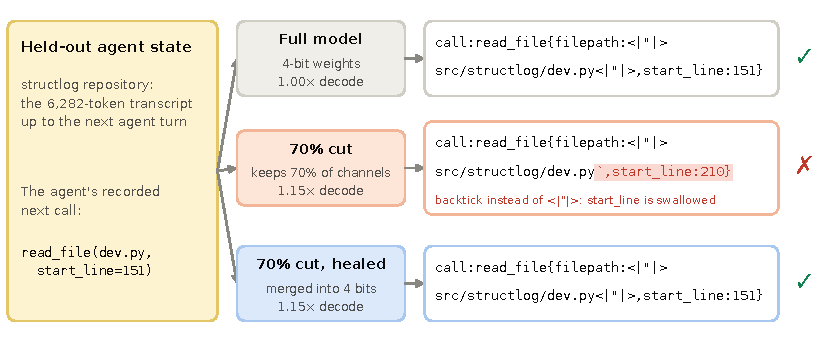
\includegraphics[width=0.9\textwidth]{fig_teaser.pdf}
  \caption{One held-out agent state, three models. The 70\% cut (70\% of MLP channels kept) ends the path with a
  backtick instead of Gemma's string delimiter \code{<|"|>} and swallows \code{start\_line}. Healed and merged, it
  writes the full model's call.}
  \label{fig:teaser}
\end{figure*}

\section{Introduction}\label{sec:intro}

An agent that writes fewer tokens per step, or writes each faster, gets more steps under a clock. Does it solve more
tasks? We pulled two levers on seconds per step, fine-tuning and pruning (Figure~\ref{fig:framework}). How the agent
reasons, writes tool calls and stops outweighed every gain in model speed we measured. Our contributions:
\begin{enumerate}
  \item Fine-tuning moves reasoning length before decisions. A teacher at the agent's decision points shortened steps
  and broke stopping.
  \item An agent-chosen cut has the 4-bit loss and speed that its bf16 mask and bytes predict, yet fails through
  malformed tool calls (Figure~\ref{fig:teaser}) that average per-token loss ranks but does not locate.
  \item Healed from the full model and merged into the 4-bit weights by stochastic rounding, the cut keeps its speed and
  stays within noise of the full model's task rate.
  \item We measure agents under noise with an A/A floor, a same-session comparison of checkpoints and a next-action
  test.
\end{enumerate}

\section{Setting}\label{sec:setting}

\paragraph{Harness.} The competition's harness~\citep{google2026gemma4competition} compiles a declarative agent (YAML,
prompts, optional LoRA~\citep{hu2021lora} adapters) and runs it in a sandbox holding the repository at its pre-fix
commit, with shell, file, edit, patch and three code-graph tools. Hidden tests grade the agent's diff, submitted or not,
as in SWE-bench~\citep{jimenez2023swebench}. We allow each \emph{episode} (one attempt at a task) 8 minutes and 24 tool
calls, a 4,096-token thinking budget and temperature 0.2. At 14,336 tokens the model summarizes older events
(compaction). Evaluation repositories are outside our training pools (two, found later under other owners, change no
result). The scorer serves one 4-bit (W4A16) checkpoint with LoRA adapters under 3\,GiB, so a pruned model cannot be
submitted. We therefore study pruning for self-hosted agents on the competition's model, harness, hardware and clock.

\paragraph{Hardware and clocks.} Training ran on a TPU v5e-8, serving on 4\X\,L4 with vLLM~\citep{kwon2023efficient}
(tensor parallel 4) and the competition's checkpoint of Gemma~4 31B~\citep{gemmateam2026gemma4}, which has one scale
per 32 inputs. \emph{Paired sessions} (Section~\ref{sec:finetune}) put two arms on one server, 8 concurrent tasks
each, on a clock doubled to 16 minutes. At 16 concurrent requests a model call writing $n$ tokens takes $a + n\cdot b$
seconds (Figure~\ref{fig:framework}), and calls take 98\% of episode time. Fine-tuning acts on $n$, pruning on $b$.
For checkpoints that cannot share a server, the \emph{same-session comparison} (Section~\ref{sec:prune}) runs them one
at a time on the same tasks, 8 at once on the 8-minute clock, in ABCD-DCBA order over two blocks, so neither order nor
time favours a model.

\begin{figure*}[b]   % bottom of page 2, below the text that follows the teaser
  \centering
  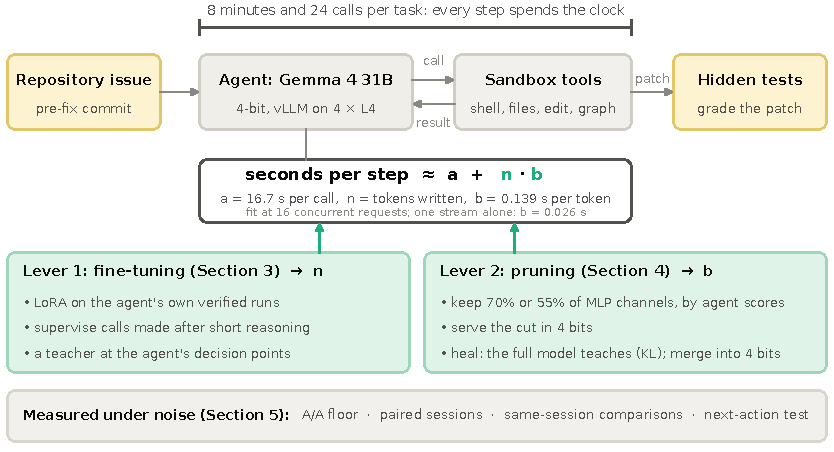
\includegraphics[width=0.8\textwidth]{fig_framework.pdf}
  \caption{The agent under the clock and the two levers.}
  \label{fig:framework}
\end{figure*}

\section{Lever 1: fine-tuning moves length first}\label{sec:finetune}

\paragraph{Pipeline.} We ran Gemma through the harness in private Kaggle Benchmarks~\citep{kaggle2025benchmarks} tasks
on SWE-rebench-style~\citep{badertdinov2025swerebench} task banks and FreshSWE-Py (issues filed after the model's
cutoff), excluding the public (development) repositories, and kept the 732 trajectories whose diffs passed the hidden
tests. Each is re-rendered as the scorer sees it. A compaction simulator matched the token counts of all 82 captured
scorer requests, and Gemma writes the summaries. A rank-16 LoRA on all projections is trained on TPU
(JAX/Tunix~\citep{google2025tunix}, fp32 factors) with the loss on tool-call bodies only. Table~\ref{tab:adapters}
lists the adapters.

\begin{table*}[t]
  \centering
  \caption{Fine-tuned adapters against the base model: step length and tasks solved. Each adapter is named after what it supervises.}
  \label{tab:adapters}
  \small
  \setlength{\tabcolsep}{4pt}
  \begin{tabularx}{\textwidth}{@{}l>{\raggedright\arraybackslash}p{2.2in}>{\raggedright\arraybackslash}p{1.15in}%
    >{\raggedright\arraybackslash}X@{}}
    \toprule
    Adapter & Data and supervision & Step text vs base (p90, full sessions) & Solved vs base (discordant:
    only-this\,/\,only-base) \\
    \midrule
    \ad{Imitation} & Stronger models' trajectories, whole turns & 0.24\X & 16 vs 26 of 103 (4/14), $p=0.031$ \\
    \ad{Thought-first} & Own runs, only turns opening with a thought & 1.72\X & 19 vs 27 (0/8), $p=0.008$ \\
    \ad{Every-call} & Own runs, compaction-aware, every call & 1.11\X & 16 vs 22 (2/8) \\
    \textbf{\ad{Short-thought}} & \ad{Every-call}'s rows, calls after thoughts $\leq$\,1,500 chars & \textbf{0.90\X} & \textbf{25 vs 18 (8/1),
    \textit{p}\,=\,0.039}; unseen: 17~vs~19 of~64~(2/4) \\
    \ad{Short-thought+} & \ad{Short-thought}'s recipe, $+153$ runs & 1.03\X\ of \ad{Short-thought} & dev: 18 vs \ad{Short-thought} 18; unseen: 27~vs \ad{Short-thought}~35 of 125~(1/9),
    $p=0.021$ \\
    \bottomrule
  \end{tabularx}
\end{table*}

\paragraph{Length moved in both directions.} \ad{Imitation} wrote short narrated thoughts and looped (26 consecutive re-reads of
one file) while its validation loss fell from 1.05 to 0.37. \ad{Thought-first} trained only on turns that opened with a thought, which
selected long ones. Served, it thought long on every turn, made 1,171 model calls to the base's 1,709 in the same time,
and lost eight tasks without winning one.

\paragraph{One filter reversed \ad{Every-call}'s longer steps.} With \ad{Every-call}'s rows and hyperparameters, \ad{Short-thought} supervised a call only
if at most 1,500 characters of reasoning preceded it (59\% of calls): shorter steps, timeouts 38 to 24, and 25 vs 18
solved. No reasoning token was trained, so length moved only through which calls were supervised. Our reading is that
the adapter generalizes the deliberation that preceded them. The gain is exploratory. On unseen repositories \ad{Short-thought} tied
the base (Table~\ref{tab:adapters}), with 90th-percentile steps still 0.89 times the base's, and more data (\ad{Short-thought+}) lost there (77
timeouts vs \ad{Short-thought}'s 53), as on the public leaderboard (\ad{Short-thought} 0.18, \ad{Short-thought+} 0.10, base 0.15).

\paragraph{A teacher at decision points.} At 717 agent states (Figure~\ref{fig:teaser}), mostly from slow or failed episodes,
the stronger Gemini 3.8 Flash judged Gemma's next step or wrote its own (589 preference pairs, \$9.21). Trained from the
base (\ad{Teacher-DPO}), Gemma took the teacher's style (90th-percentile step 172 tokens, \ad{Short-thought}'s 514) but looped (36 of 98 episodes)
and lost to \ad{Short-thought} (20 vs 27). A second stage on \ad{Short-thought} computed the preference in each training step (\ad{Teacher-DPO-2},
DPO~\citep{rafailov2023direct} plus a next-token loss on the teacher's step). It removed the losses to \ad{Short-thought} (20 vs 17,
5/2) and kept steps short (229 vs 610 tokens, 56 vs 125\,s at the 90th percentile). Yet the agent was not faster. Once a
patch is submitted, an episode ends at the first response without a tool call, and \ad{Teacher-DPO-2}, after submitting early, kept
calling tools until the clock. Of its episode time, 52\% came after a first patch that then changed in 1 of 65
episodes. The next-token loss alone kept steps short and stops normal, but the agent looped (31 of 103). The teacher's
data shortens steps, and the preference term prevents loops but breaks the stop.

\section{Lever 2: prune what the agent does not use}\label{sec:prune}

Each of the model's 60 layers has a gated MLP with 21,504 hidden channels (about 70\% of the layer's weights). We score
each channel by the RMS of its activation over 300 agent trajectories (2.37\,M tokens) times the norm of its
down-projection weights. A cut is an exact mask, without retraining. Its \emph{damage} is the rise in nats per token on
\emph{agent tokens}, the thought and call of each short-reasoning turn (at most 1,500 characters of reasoning, 17\% of
the agent's text), in 40 held-out trajectories from other tasks. The 70\% cut (70\% of channels kept per layer, 21\% of
layer weights removed) costs $+0.080$ with agent scores, $+0.867$ with WikiText-103 scores and $+0.533$ at random.

\paragraph{Real 4-bit cuts.} We cut the competition's 4-bit checkpoint and served each cut in vLLM. Single channels
split the down projection's quantization groups of 32, so the projection is re-quantized (activation-weighted) or cut in
whole groups. The 85\%, 70\% and 55\% cuts decode 1.05, 1.15 and 1.24 times faster (1.03-1.14 at 8 streams) for a
served damage of $+0.025$, $+0.084$ and $+0.188$ (Appendix~\ref{app:cuts}). Removing 6 layers by block
influence~\citep{men2024shortgpt} costs $+0.925$ at 1.07\X\ (Figure~\ref{fig:speed}). Every single-channel cut loses
in vLLM what its bf16 mask predicted, within 0.005 nats. Whole groups lose twice as much.

\begin{figure}[!htb]
  \centering
  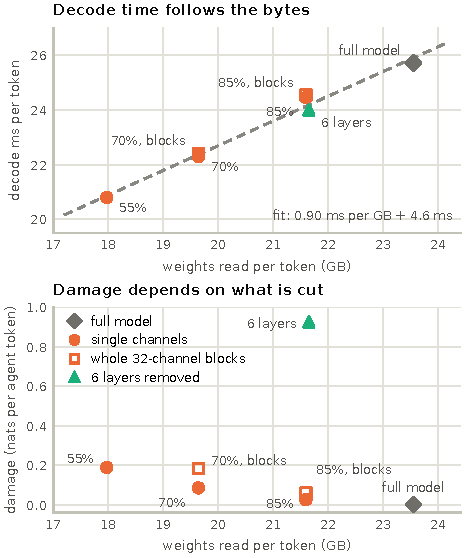
\includegraphics[width=\linewidth]{fig_speed.pdf}
  \caption{Decode time follows the bytes read (top). At equal bytes, damage depends on what is removed (bottom).}
  \label{fig:speed}
\end{figure}

\paragraph{Tasks under the clock.} In the same-session comparison (112 unseen-repository tasks,
Figure~\ref{fig:tasks}), the 70\% cut solved 20 tasks against 32 and 34 for two runs of the full model, which differed
on only 8 tasks (3/5). The cut won none of the 12 and 14 tasks that separated it from them (exact paired sign-flip
test, $p=1.5\times10^{-5}$), in both task blocks and both orders. It lost them at the clock (72 timeouts against
43-44), and none of our 1,944 timed-out episodes passed the hidden tests. The failure is in the call syntax
(Figure~\ref{fig:teaser}): a string closed with a backtick or a JSON quote instead of Gemma's delimiter swallows the
next argument. Of the cut's calls, 24\% were malformed, against 2-3\% for the full model. The call fails, the agent
resends it, and 42 episodes looped, 31 until the clock (full-model runs: 4 and 7).

\begin{figure}[!htb]
  \centering
  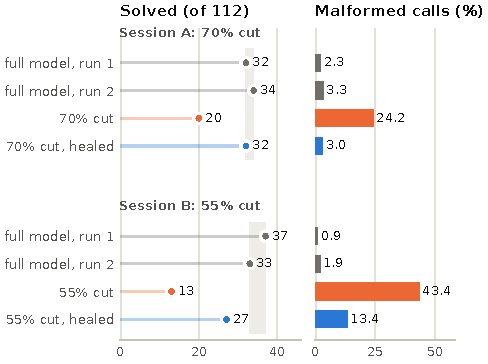
\includegraphics[width=\linewidth]{fig_tasks.pdf}
  \caption{Same-session comparisons on 112 unseen-repository tasks. Grey band: two runs of the full model.}
  \label{fig:tasks}
\end{figure}

\paragraph{Healing from the full model (mask and adapter off).} A rank-16 LoRA is trained for two epochs on 628 agent
trajectories in two arms on identical batches. The KL arm minimizes $\mathrm{KL}(\text{full}\,\|\,\text{cut})$ at
every token, the next-token arm the next-token loss. A removed channel gets no gradient, so the adapter slices exactly
onto the 4-bit cut. The KL arm met its pre-registered bar, damage below $+0.04$ and KL halved (2.4 TPU hours). In the
trainer's bf16 evaluation the damage fell from $+0.085$ to $+0.021$ and the KL on agent tokens from 0.098 to 0.042. The next-token arm reached
$-0.078$, below the full model, while its KL rose to 0.243. It fit the data, not the model. Served through vLLM's LoRA
path, the adapter costs the whole speedup (1.02\X\ against 1.15\X). Rounding $W + dW$ to the nearest 4-bit value would
erase the repair, since its deltas average 5\% of a grid step (Scale-QLoRA~\citep{li2026scaleqlora} saw the same). So
we use stochastic rounding~\citep{gupta2015deep} (up or down at random, exact in expectation), and the merged cut keeps
the repair ($+0.022$ nats) and the speed (1.15\X).

In the same-session comparison the merged cut solved 32 of 112, within noise of the full model ($-1$ task, 95\%
interval $-7.5$ to $+5$, discordant 5/5 and 6/8; against the unhealed cut 15/3, $p=0.0075$). It made 3\% malformed
calls and 36 timeouts against 43-44 (seven fewer, worth about 3 tasks, since full-model episodes ending after 7 minutes
pass 43\% of the time). Its calls took 16.9\,s against 19.0-19.3\,s at equal length. On the 55\% cut (1.24\X),
healing recovers the same share of the damage ($+0.185$ to $+0.047$, missing its $+0.04$ bar) and 14 of the 22 lost
tasks, still short of the full model ($p=0.007$). Malformed calls fell from 43\% to 13\% (full model 1-2\%,
Figure~\ref{fig:tasks}).

\paragraph{A next-action test.} At 102 held-out agent states (starts of short-reasoning turns in 40 trajectories), each
model's greedy next call is compared with the full model's (Figure~\ref{fig:nextaction}). Two engines with the same
weights agree on 78\% of calls, sampling at the agent's temperature on 64\%, and the cuts, healed or not, on 28-42\%.
Exact agreement does not track tasks (the cuts solving 20 and 13 agree on 29\% and 28\%). The malformed share does, and
so does agreement with the call the agent recorded (full 0.40, healed 0.34, 70\% 0.28, 55\% 0.24). The test is a gate,
not a predictor.

\begin{figure}[!htb]
  \centering
  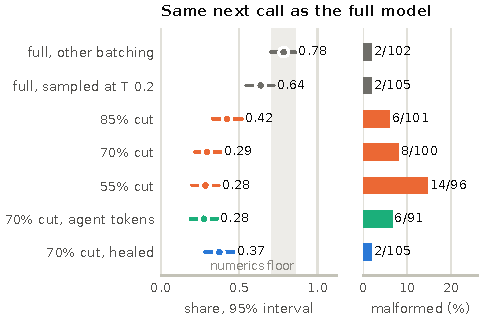
\includegraphics[width=\linewidth]{fig_nextaction.pdf}
  \caption{The next-action test at 102 held-out states. Grey band: two engines with the same weights.}
  \label{fig:nextaction}
\end{figure}

\paragraph{Two scores for pruning reasoning.} Scoring channels only on agent tokens, in the spirit of RAC's calibration
on the model's own chains~\citep{lucas2025reasoning}, changed nothing at 70\% (Figure~\ref{fig:nextaction}). Scoring
by token role (after SKIM~\citep{choi2026skim}, Section~\ref{sec:related}) gives an equal vote to text read, prose,
argument values, call syntax and the closing quote (0.08\% of positions). Split by role, the 55\% cut's loss rose most
on that quote ($+0.50$ nats, against $+0.19$ overall). At 141 states the role-scored cut halved both that rise and the
wrongly closed strings, but its calls lost their opener (their first token) instead (Figure~\ref{fig:failure}). In
all, 20\% of its attempts failed against 19\% (pre-registered test, parsed calls only: 11\% vs 16\%, $p=0.14$). A
format-enforcing grammar would block the failures the role score adds but not those it removes (inference).

\begin{figure}[!htb]
  \centering
  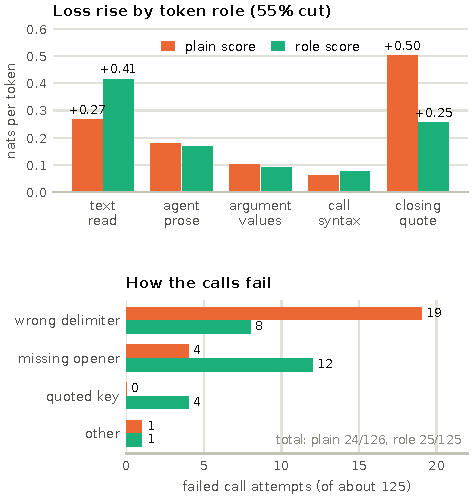
\includegraphics[width=\linewidth]{fig_failure_moves.pdf}
  \caption{Scoring by token role (55\% cut, 141 states). The closing quote recovers and the opener breaks.}
  \label{fig:failure}
\end{figure}

\paragraph{Speed without a cut.} N-gram speculative decoding~\citep{saxena2023prompt} kept the full model's calls (89\%
the same next call, malformed 2/103) but sped up real agent turns only 1.05-1.07\X. Unlike a cut's, its gain depends on
the text (3.4\X\ on a synthetic continuation, Figure~\ref{fig:speculation}). We did not test Gemma~4's own draft model,
a multi-token-prediction (MTP) drafter~\citep{gemmateam2026gemma4}.

\begin{figure}[!htb]
  \centering
  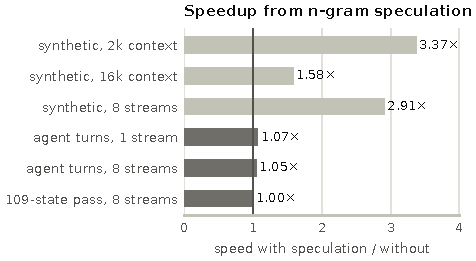
\includegraphics[width=\linewidth]{fig_speculation.pdf}
  \caption{N-gram speculative decoding against plain decoding (full model, same session).}
  \label{fig:speculation}
\end{figure}

\section{Measuring agents under noise}\label{sec:noise}

\paragraph{Pairing and the noise floor.} Between sessions the same model moved by up to ten tasks and flipped 7-14\% of
the same unseen tasks. Paired sessions, compared by discordant tasks (exact McNemar), separated adapters. Two identical
full-model arms on one server, the A/A floor, flipped 6 of 82 tasks (2/4), as many as across sessions. Pairing
controls load and time of day but leaves the flips, so only lopsided splits such as 8/1 carry signal.

\paragraph{Exploratory and confirmatory.} Single-session $p$-values near 0.04, among about twenty adapter comparisons,
are exploratory, and we claim only directions that held across sessions or mechanisms. The same-session, role and
speculation tests are confirmatory, with analysis set, primary test and gates fixed before each run.

\section{Related work}\label{sec:related}

Fine-tuning on a model's own filtered successes dates to expert iteration~\citep{anthony2017thinking},
STaR~\citep{zelikman2022star} and ReST-EM~\citep{singh2023beyond}. SWE-Gym~\citep{pan2024training} found it weak for
software agents. SWE-smith~\citep{yang2025swesmith}, R2E-Gym~\citep{jain2025r2egym} and
SWE-rebench~\citep{badertdinov2025swerebench} supply tasks. \citet{cuadron2025danger} measured overthinking in agents,
and On the Clock~\citep{wang2026clock} agents under wall-clock budgets. Our preference stages use
DPO~\citep{rafailov2023direct} and IPO~\citep{azar2023general}. \ad{Teacher-DPO}'s collapse matches likelihood
displacement~\citep{razin2024unintentional}.

Perplexity misses what compression breaks~\citep{jaiswal2023compressing}, for agents too
(ACBench~\citep{dong2025compressed}, worst on JSON outputs), and flips and KL track it better~\citep{dutta2024accuracy}.
Quantization amplifies agents' existing failures~\citep{jang2026flat}, and we trace them to call syntax. Our channel
score is a structured Wanda~\citep{sun2023simple}, FLAP's Wanda-sp~\citep{an2023fluctuation}. Reasoning models are
pruned with calibration on their own chains (RAC~\citep{lucas2025reasoning}, SSGR~\citep{xiang2025think},
RESP~\citep{wang2025think}, OBC-Prune~\citep{nguyen2026obcprune}), without tools or a clock. Concurrent work,
SKIM~\citep{choi2026skim}, prunes tool-calling agents by per-role saliency and heals on-policy, under a grammar that
enforces the format.

Minitron~\citep{muralidharan2024compact} is our cut-then-distil template. LLM-Pruner~\citep{ma2023llmpruner} retrains,
D-Pruner~\citep{zhang2024pruning} calibrates on a target domain, and self-data
distillation~\citep{thangarasa2024selfdata} heals with the unpruned model's outputs. We heal with an off-policy forward
KL \citep[on-policy:][]{agarwal2023onpolicy,gu2023minillm} and merge by stochastic rounding, whereas
QA-LoRA~\citep{xu2023qalora} trains merge-ready adapters and PEQA~\citep{kim2023memory} tunes the quantization scales.
Speculative decoding~\citep{leviathan2022speculative,chen2023accelerating} speeds decoding without changing the model,
and SuffixDecoding~\citep{oliaro2024suffixdecoding} targets agents. On error bars, see \citet{miller2024adding}. Agent
reruns vary by 2-6 points~\citep{bjarnason2026randomness}.

\paragraph{Further related work.} Nested models such as MatFormer~\citep{devvrit2023matformer} and Star
Elastic~\citep{taghibakhshi2026starelastic}, which also works in 4 bits, are trained to be cut. Ours was cut post hoc.
Pruning degrades tool-call arguments before intent~\citep{zhang2026breaks}. In the study of \citet{jang2026flat},
agents' scores stay flat while 4-bit quantization amplifies their existing failures. Under our clock, the amplified
failure cost tasks. Scale-QLoRA~\citep{li2026scaleqlora} also finds that stochastic re-rounding collapses QAT-LoRA
adapters, but those adapters are trained for a nearest-rounding grid, a different case from our single unbiased merge
of an adapter trained in floating point. ActionOPD~\citep{yuan2026actionopd} distils a black-box teacher's decisions at
the states a student visits. Kaggle's staff call competitions the gold standard of evaluation~\citep{sculley2025position},
and Google deploys repair agents under latency limits~\citep{ziftci2026catching}.

\section{Limitations and conclusion}\label{sec:conclusion}

With one model, harness and competition, the mechanisms (supervised actions condition reasoning length, cuts break rare
syntax tokens, preference terms move stopping) may generalize but the numbers need not. The fine-tuning gain held on
development repositories only. We did not try policy-gradient training. Each cut has one mask and one healing run. The
token-level tests cover short-reasoning turns within 8,192 tokens, on held-out tasks that share repositories with
training rows. No affordable control changes time with behaviour fixed. The healed cut's result is one session of 112
tasks, at our own load of 8 tasks at a time, not a documented scorer setting.

Before asking what a faster model buys an agent, measure the agent: its tokens per step, which fine-tuning moves first,
and its time per token, which follows the bytes read. Before any long run, check cheaply whether it still writes its
calls and stops as it did. On a clock, those decided every result we measured. Healed by its full model, the 70\% cut
chosen by the agent's use stayed within noise of the full model's task rate at 1.15 times its decode speed, but the
55\% cut did not.

\section*{Code and data}
The code, the result files and this paper's sources are at \url{https://github.com/wilmerhenao/under-the-clock}: the
code that builds the training rows, trains the adapters, scores, cuts, heals and serves the pruned models, and
analyses the runs; the small result files behind every number here; and the script that draws the figures from them.
Every experiment ran as a Kaggle notebook. Appendix~\ref{app:notebooks} lists them, and the repository's README maps
each number to a notebook version and a result file. Task data, agent trajectories and model weights are not
redistributed: the notebooks rebuild or load them from their sources.

\section*{Disclosure}
This work was done independently, outside the author's role at Invesco, and used no Invesco resources. The views
expressed are the author's own and not necessarily those of Invesco.

\bibliographystyle{plainnat}
\bibliography{refs}

\clearpage
\appendix

\section{Real 4-bit cuts}\label{app:cuts}

Table~\ref{tab:cuts} gives the measurements behind Figure~\ref{fig:speed}. The model is Gemma~4 31B in W4A16
(compressed-tensors, group 32), served by vLLM on 4\X\,L4. Decode speed is for one stream at a 2,000-token prompt, and
``8 streams'' is the total decode rate of eight 2,000-token prompts at once. Damage is the rise in held-out nats per
token on the agent's own text (40 trajectories, 25,896 tokens). ``Predicted'' is the bf16 mask's damage before any
4-bit serving.

\begin{table}[!ht]
  \centering
  \caption{Real 4-bit cuts: weights read, decode speed and damage. Speeds are relative to the full model's 38.9 tok/s
  on one stream and 210 tok/s on 8.}
  \label{tab:cuts}
  \small
  \setlength{\tabcolsep}{3.5pt}
  \begin{tabular*}{\columnwidth}{@{\extracolsep{\fill}}lrrrrr@{}}
    \toprule
    & & \multicolumn{2}{c}{Decode speed} & \multicolumn{2}{c}{Damage} \\
    \cmidrule(lr){3-4}\cmidrule(l){5-6}
    MLP kept & GB & 1 stream & 8 streams & served & predicted \\
    \midrule
    100\% & 23.5 & 1.00\X & 1.00\X & 0 & 0 \\
    85\% & 21.6 & 1.05\X & 1.03\X & $+0.025$ & $+0.025$ \\
    70\% & 19.6 & 1.15\X & 1.09\X & $+0.084$ & $+0.080$ \\
    55\% & 18.0 & 1.24\X & 1.14\X & $+0.188$ & $+0.185$ \\
    6 layers$^{a}$ & 21.6 & 1.07\X & 1.09\X & $+0.925$ & $+0.970$ \\
    \bottomrule
  \end{tabular*}
  \par\smallskip
  {\footnotesize\raggedright $^{a}$Removed by block influence~\citep{men2024shortgpt}. The other rows keep that share of
  MLP channels in every layer.\par}
\end{table}

\section{Notebooks}\label{app:notebooks}
\raggedright   % notebook names break at any character in a 3.25in column: ragged, not stretched

Each experiment ran as a Kaggle notebook at \url{https://www.kaggle.com/code/verracodeguacas/} followed by the name
below (each name links to its notebook). The repository's README gives the version behind each number and its result
files.

\paragraph{Fine-tuning (Section~\ref{sec:finetune}).} The compaction simulator: \nb{g4dev-train-mix4-cpu}. The
training rows are private Kaggle datasets (\nolinkurl{g4dev-g11-data}, \nolinkurl{g4dev-g13-data}), since they hold agent
trajectories; the repository's scripts render them from the agent's runs. The teacher's labels:
\nb{g4dev-g17-labels-cpu}.
Trainers: \ad{Imitation}, \nb{g4dev-train-g2b-gpu} (also its evaluation); \ad{Thought-first}, \nb{g4dev-train-g6-gpu};
\ad{Every-call}, \nb{gemma-4-31b-agent-lora-compaction-aware-trainer}; \ad{Short-thought},
\nb{gemma-4-31b-agent-lora-short-thought-trainer}; \ad{Short-thought+},
\nb{gemma-4-31b-agent-lora-short-thought-trainer-v3}; \ad{Teacher-DPO},
\nb{gemma-4-31b-agent-teacher-guided-step-preferences}; \ad{Teacher-DPO-2},
\nb{gemma-4-31b-agent-in-step-teacher-preferences}. Paired sessions on the development repositories:
\nb{g4dev-eval-g6-gpu}, \nb{g4dev-eval-g10a-gpu}, \nb{g4dev-eval-g11a-gpu}, \nb{g4dev-eval-g11g13-gpu}. On unseen
repositories: \nb{g4dev-eval-rg-base-g11a-gpu}, \nb{g4dev-eval-rg-g11g13-gpu}, \nb{g4dev-eval-rg-g17-gpu},
\nb{g4dev-eval-rg-g17v2a-gpu}, \nb{g4dev-eval-rg-g17v2b-gpu}. The A/A floor: \nb{g4dev-eval-rg-aa-gpu}.

\paragraph{Pruning (Section~\ref{sec:prune}).} Channel scores and damage: \nb{g4dev-prune-score-gpu},
\nb{g4dev-prune-score3-gpu}; the role score: \nb{g4dev-prune-score4-gpu}. Real 4-bit cuts and decode speed:
\nb{g4dev-prune-serve-gpu}. Healing: \nb{gemma-4-31b-agent-pruned-model-teacher-healing} (70\%),
\nb{gemma-4-31b-agent-healing-a-deeper-pruning-cut} (55\%). The LoRA serving path: \nb{g4dev-prune-serve2b-gpu}.
Merged healing and the next-action test: \nb{g4dev-prune-serve5-gpu}. The role score's test: \nb{g4dev-prune-serve6-gpu}.
Speculative decoding: \nb{g4dev-prune-serve7-gpu}. Same-session comparisons: \nb{g4dev-eval-rg-same4-gpu} (70\%),
\nb{g4dev-eval-rg-same55-gpu} (55\%).

\end{document}
